% Regenerate from this directory:
% latex -interaction=nonstopmode -halt-on-error hill-climbing.tex
% dvisvgm --no-fonts --exact --bbox=papersize -o hill-climbing.svg hill-climbing.dvi
\documentclass[tikz,border=8pt]{standalone}
\begin{document}
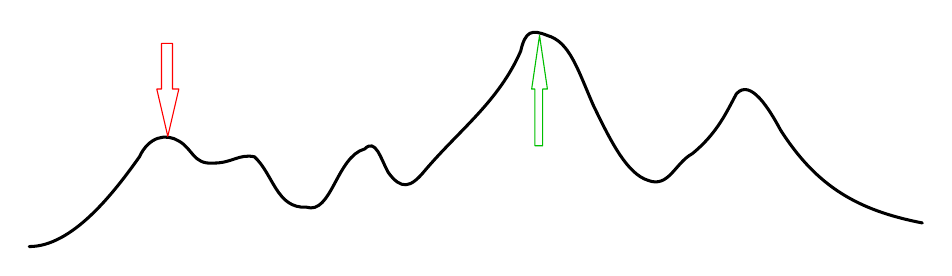
\begin{tikzpicture}[x=.02cm,y=-.02cm,line join=round,line cap=round]
  % A multimodal objective. The first peak is a local maximum;
  % the highest peak is the global maximum.
  \draw[line width=1.1pt]
    (59,197)
    .. controls (86,197) and (112,164) .. (129,140)
    .. controls (135,127) and (146,125) .. (154,130)
    .. controls (163,135) and (163,145) .. (176,144)
    .. controls (188,144) and (192,138) .. (202,140)
    .. controls (214,151) and (216,173) .. (235,172)
    .. controls (251,177) and (254,140) .. (272,135)
    .. controls (279,128) and (282,141) .. (287,150)
    .. controls (295,161) and (301,160) .. (310,149)
    .. controls (332,123) and (357,105) .. (371,73)
    .. controls (374,60) and (378,59) .. (388,63)
    .. controls (402,67) and (407,84) .. (417,107)
    .. controls (429,132) and (439,151) .. (452,155)
    .. controls (465,160) and (469,144) .. (480,138)
    .. controls (496,125) and (502,111) .. (508,100)
    .. controls (517,90) and (529,110) .. (536,123)
    .. controls (559,159) and (585,174) .. (626,182);
  % Red downward arrow: a local optimum reached by hill climbing.
  \draw[red,line width=.4pt]
    (143,68) -- (150,68) -- (150,97) -- (154,97)
    -- (147,127) -- (140,97) -- (143,97) -- cycle;
  % Green upward arrow: the global optimum.
  \draw[green!75!black,line width=.4pt]
    (380,133) -- (385,133) -- (385,97) -- (388,97)
    -- (383,63) -- (378,97) -- (380,97) -- cycle;
\end{tikzpicture}
\end{document}
